
Oscillations are commonplace when discussing a physical system in a stable equilibrium being subject to displacements. Simple harmonic motion can be estimated for small displacements, making them extremely widespread.

A mass on the end of a spring (along the x-axis) is an example of simple harmonic motion and is subject to Hooke's Law, namely, $F_x(x) = -kx$. This force caused by Hooke's Law if considered a {\itshape restoring force}, that is, returning the object back to an equilibrium (in this case, $x=0$).

The potential energy from this force (recall: $\int F(x) dx = U(x)$) is $U(x) = \frac{1}{2}kx^2$. The graph of $x vs U(x)$ (figure \ref{fig:SHO_xvsE}) tells the biggest story. It shows a parabola that oscillates between two amplitudes of oscillation $-A$ and $A$ with a maximum energy of $E$.

Examining simple harmonic motion using Newton's laws for a mass $m$ displaced from a position $x$ of stable equilibrium, like a cart on a frictionless (more on damped later) spring. The only applicable force is the restoring spring force, $F_x(x) = -kx$. Thus, the equation of motion is $m \ddot{x} = F_x = -kx$ or

\begin{equation*}
    \ddot{x} = -\frac{k}{m}x = \omega^2x.
\end{equation*}

\noindent where the constant $\omega = \sqrt{\frac{k}{m}}$ is the angular frequency with which the cart will oscillate. This expression and the subsequent solutions are useful beyond strict one dimensional analyses. They are also useful for skateboards on half pipes, where $\ddot{\phi} = -\omega^2\phi$. There are four different (each important) versions of the same solution, as shown below.

\begin{figure}[h]
    \centering
    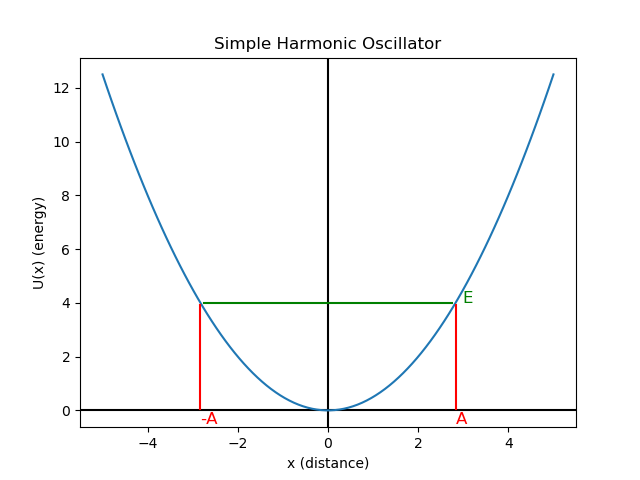
\includegraphics[width=13cm]{Classical_Mechanics/2.10-SHO/SHO_xvsE.png}
    \caption{Shows the oscillation of a mass on a spring. As $U \rightarrow E$, all energy is converted to potential energy (from kinetic) and mass retracts back to equilibrium. The two turning points are $x=\pm A$. Solving for $A$ yields $\pm \sqrt{8} \approx 2.8284 \dotsc$.}
    \label{fig:SHO_xvsE}
\end{figure}


{\bfseries \noindent The exponential solutions}

The above equation of motion is a linear, second-order, homogeneous differential equation and so has two independent solutions. The most convenient solutions are $x(t) = e^{i \omega t}$ and $x(t) = e^{-i \omega t}$. The sum of these solutions is a solution (due to the superposition principle) along with any constant multiples of each,

\begin{equation*}
    x(t) = C_1  e^{i \omega t} + C_2  e^{-i \omega t}
\end{equation*}

Any solution can be expressed in the form above with subtle use of $C_1$ and $C_2$. This is often the best solution to use.


{\vspace{0.35cm} \bfseries \noindent The sine and cosine solutions}

Using Euler's formula, we can rewrite $x(t)$ as $C_1 (cos(\omega t) + i sin(\omega t)) + C_2  (cos(\omega t) - i sin(\omega t))$. This yields,

\begin{equation*}
    x(t) = (C_1 + C_2)cos(\omega t) + i(C_1 - C_2)sin(\omega t)
\end{equation*}

\noindent where we can substitute new coefficients in for the old ones: $B_1 cos(\omega t) + B_2 sin(\omega t)$. This represents simple harmonic motion: any motion that is a combination of sines and cosines. $B_1$ and $B_2$ are determined using the initial conditions of the system.

Note that, since sine and cosine are both periodic, the system is periodic as well. This is given as

\begin{equation*}
    \tau = \frac{2 \pi}{\omega} = 2\pi \sqrt{\frac{m}{k}}.
\end{equation*}


{\vspace{0.35cm} \bfseries \noindent The phase-shifted cosine solutions}

Our previous solution with a real cosine and complex sine is difficult to imagine physically, therefore we can rewrite it: first, set $A = \sqrt{B_1^2 + B_2^2}$ - this is a right triangle with sides $B_1$ and $B_2$ with hypotenuse $A$ and an arbitrary angle $\delta$ between lengths $B_1$ and $A$. Now rewrite,

\begin{gather*}
    x(t) = A [\frac{B_1}{A}cos(\omega t) + \frac{B_2}{A} sin(\omega t)] \\
    = A[cos(\delta) cos(\omega t) + sin(\delta) sin(\omega t)] \\
    = A cos(\omega t - \delta)
\end{gather*}

It is clear that the cart (or any mass) is oscillating with amplitude $A$, but is also shifted in phase by $\delta$. So, when $t=0$, the cosine argument is now $-\delta$ causing the oscillation to lag behind the normal cosine oscillation.


{\vspace{0.35cm} \bfseries \noindent The real part of a complex exponential solutions}

The final useful way to write the solution is in terms of the complex exponentials found in the first solution. Taking $x(t)$ and solving for $C_1$ and $C_2$ in terms of the coefficients $B_1$ and $B_2$ are $C_1 = \frac{1}{2}(B_1 - i B_2)$ and $C_2 = \frac{1}{2}(B_1 + i B_2)$. It is obvious that $C_1^* = C_2$ (complex conjugate) and that the second term in,

\begin{equation*}
    x(t) = C_1 e^{i \omega t} + C_1^* e^{-i \omega t}
\end{equation*}

\noindent is simply just the complex conjugate of the first. Now, $z + z^* = 2 Re z$, so,

\begin{equation*}
    x(t) = Re C e^{i \omega t} = Re A e^{i(\omega t - \delta)}.
\end{equation*}

This result is best thought of in complex space: while the complex number moves around in a circle, (x: real, y: complex) the x-axis is simply a projection of the complex number above on the real axis, namely the phase-shifted cosine solution.

\vspace{0.35cm}

Considering the potential energy in these solutions, 

\begin{equation*}
    U = \frac{1}{2}kx^2 = \frac{1}{2}k A^2 cos^2(\omega t - \delta).
\end{equation*}

Then solving for the kinetic energy (requires differentiation of $x(t)$), 

\begin{equation*}
    T = \frac{1}{2}m \dot{x}^2 = \frac{1}{2}m \omega^2 A^2 sin^2(\omega t - \delta) = \frac{1}{2}k A^2 sin^2(\omega t - \delta).
\end{equation*}

\noindent where $\omega^2$ is replaced by $\frac{k}{m}$. Both energies oscillate between $0$ and $\frac{1}{2}k A^2$ and are perfectly out of phase and the total energies constant at $\frac{1}{2}k A^2$ because it is conservative.
